%%%%%%%%%%%%%%%%%%%%%%%%%%%%%%%%%%%%%%%%%%%%%%%%%%%%%%%%%%%%%%%%%%%%%%%%%%%%%%%%%%
%%																				%%
%% File name: 		20hannes.tex												%%
%% Project name:	Hochleistungsantenne										%%
%% Type of work:	T3X00 project work											%%
%% Author:			Sarah Brückner, Maximilian Stiefel, Hannes Bohnengel		%%
%% Date:			14th May 2016												%%
%% University:		DHBW Ravensburg Campus Friedrichshafen						%%
%% Comments:		Created in gedit with tab width = 4							%%
%%																				%%
%%%%%%%%%%%%%%%%%%%%%%%%%%%%%%%%%%%%%%%%%%%%%%%%%%%%%%%%%%%%%%%%%%%%%%%%%%%%%%%%%%

\chapter{GPredict}

\section{Übersicht}

GPredict ist eine freie Software zur Satellitenverfolgung und Orbitvorhersage und steht als Quellcode oder bereits fertig kompiliertes Programm für Windows, Mac OS und Linux zur Verfügung. Die Software ist in C geschrieben und unter der GNU \ac{GPL} lizenziert, somit kann sie frei verändert und an die entsprechenden Nutzervoraussetzungen angepasst werden.\newpar
In Abbildung \ref{fig:gpredict-principle} ist das Prinzip eines Satellitenverfolgungsprogramms zu sehen (die blauen Blöcke stellen hierbei die Funktionalität des Programms dar). Zunächst wird an Hand der Keplerschen Bahnelemente und dem aktuellen Zeitpunkt die absolute Position des Satelliten berechnet. Daraufhin wird der Vektor, der von der Bodenstation zum Satelliten zeigt, bestimmt. Nun können Azimut und Elevation dieses Vektors für die Ansteuerung der Antenne verwendet werden.

\begin{figure}[h]
	\centering
	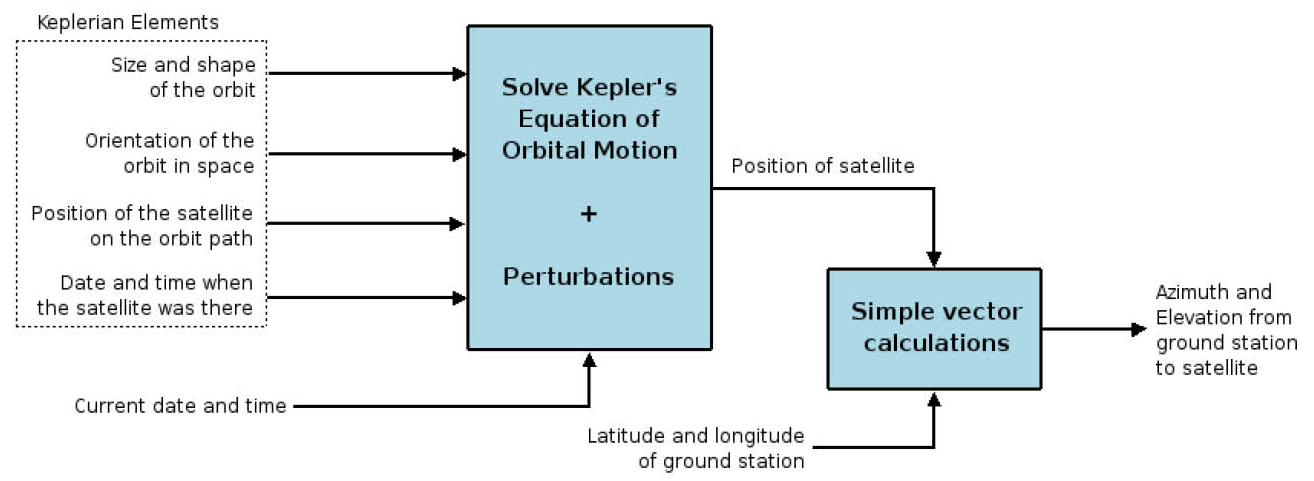
\includegraphics[width=1\textwidth]{gpredict-principle}
	\caption{Prinzip eines Satellitenverfolgungsprogramms \cite{gpredictmanual}}
	\label{fig:gpredict-principle} 
\end{figure}

Zur Berechnung der Satellitenposition wird auf den NORAD SGP4/SDP4 Algorithmus zurückgegriffen (siehe Abschnitt XXX). Um hierfür zu jedem Zeitpunkt die aktuellen Kepler-Elemente des zu verfolgenden Satelliten zu kennen, gibt es unter GPredict die Möglichkeit einer automatischen Aktualisierung über HTTP, FTP oder aus dem lokalen Verzeichnis.

\clearpage

Bei GPredict ist im Gegensatz zu anderen Satellitenverfolgungsprogrammen wie SatPC32 kein Limit an zu verfolgenden Satelliten und Bodenstationen gegeben. Durch die Verwendung von Modulen kann außerdem unkompliziert zwischen verschiedenen Konfigurationen gewechselt werden. Die Orbitvorhersage eines Satelliten lässt sich sowohl grafisch als auch tabellarisch darstellen, wobei durch die Einstellungen verschiedenster Parameter eine sehr individuelle Anzeige erreicht werden kann \cite{gpredictsource}.

\section{Grafische Oberfläche}

In Abbildung \ref{fig:gpredictstartup} ist die grafische Oberfläche von GPredict zu sehen. In der Standardkonfiguration ist dort zunächst die Kartenansicht bzw. \myemph{Map View} (oben), die Polaransicht bwz. \myemph{Polar View} (links unten) und die Einzelsatellitenansicht bzw. \myemph{Single-Satellite View} (rechts unten) zu sehen.

\begin{figure}[h]
	\centering
	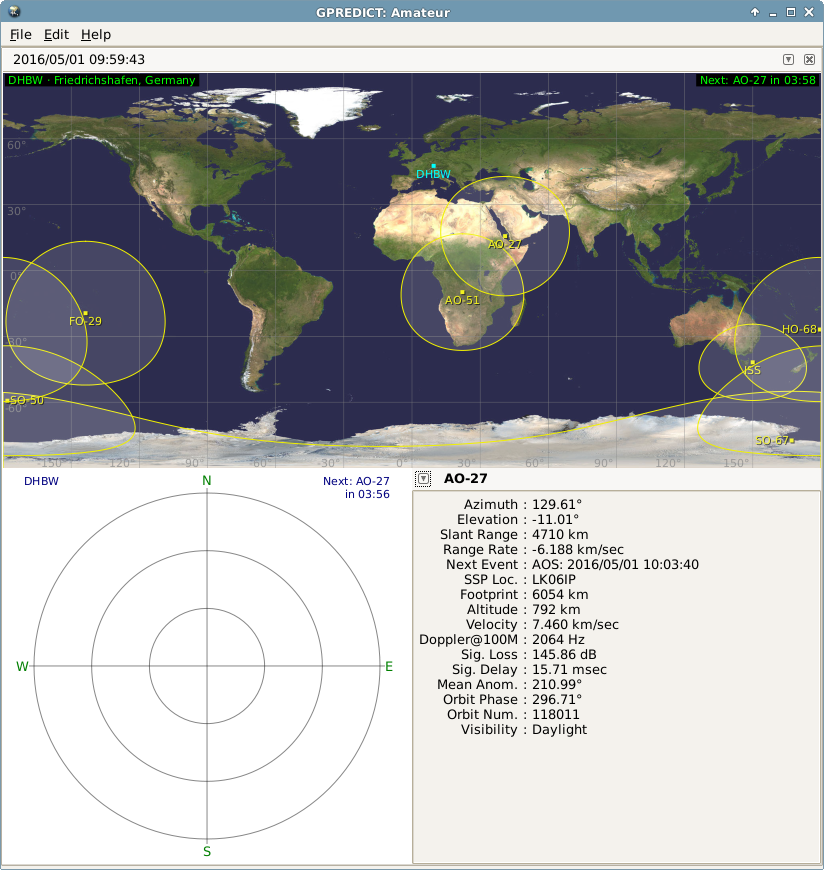
\includegraphics[width=0.75\textwidth]{gpredict-startup}
	\caption{Standardoberfläche von GPredict}
	\label{fig:gpredictstartup} 
\end{figure}

\clearpage

\subsection{Grundansichten}

Zu den oben genannten Ansichten kommen noch zwei Weitere hinzu, die Listenansicht bzw. \myemph{List View} und eine Ansicht für bevorstehende Vorbeiflüge, die sogenannte \myemph{Upcoming Passes View}. Im Folgenden werden die verschiedenen Ansichten genauer beschrieben:\newpar
\textbf{Map View}\\
Diese Ansicht besteht, wie in Abbildung \ref{fig:gpredictstartup} zu sehen, aus einer Weltkarte auf der die aktuellen Standorte der für das aktuelle Modul ausgewählten Satelliten zu sehen ist. Das heißt der Punkt auf dem der entsprechende Satellit senkrecht bezogen auf den Erdmittelpunkt steht. Außerdem ist um diesen Punkt die Fläche umrahmt, von der der Satellit von der Erde aus sichtbar ist. Mit einem Rechtsklick auf einen Satellitennamen kann außerdem die Option \myemph{Ground Track} aktiviert werden, mit welcher die Spur des Satelliten für mehrere Orbits angezeigt wird.\newpar
\textbf{Polar View}\\
Die \myemph{Polar View} (siehe Abbildung \ref{fig:gpredictstartup}) stellt eine Draufsicht auf die Bodenstation dar, bei der die Polarachse den Azimutwinkel darstellt und die Radialachse den Elevationswinkel. Mit einem Rechtsklick auf einen Satelliten lässt sich mit der Option \myemph{Show sky track} aktivieren, das die Spur des entsprechenden Satelliten anzeigt wird. Zusätzlich wird das aktuelle Modul links oben angezeigt, der nächste sichtbare Satellit (rechts oben) und die genauen Werte für Azimut und Elevation (links unten) sobald sich der Mauszeiger auf der \myemph{Polar View} befindet.\newpar
\textbf{Single-Satellite View}\\
In dieser Ansicht (siehe Abbildung \ref{fig:gpredictstartup}) werden detaillierte Informationen zu einem ausgewählten Satelliten angezeigt, z.B. Azimut, Elevation, Entfernung der direkten Sichtverbindung (\myemph{Slant Range}), Höhe, Geschwindigkeit, Dopplerverschiebung oder Signaldämpfung. Mit einem Klick auf das Dreieck links neben dem Satellitennamen kann zwischen den für dieses Modul ausgewählten Satelliten gewechselt werden.

\clearpage

\textbf{List View}\\
Die Listenansicht zeigt eine tabellarische Auflistung aller für das aktuelle Modul ausgewählten Satelliten mit verschiedenen Details, mit je einem Satelliten pro Zeile. In Abbildung \ref{fig:listview} ist die Listenansicht mit allen verfügbaren Details zu sehen. Mit einem Klick auf eine entsprechende Kategorie lässt sich das Sortierkriterium ändern. Falls hier ein variables Kriterium wie die Geschwindigkeit eingestellt wird, ändert sich die Sortierreihenfolge mit der eingestellten Auffrischrate (\myemph{Refresh Rate}). Die Bezeichnung des jeweiligen Details ist in dieser Ansicht abgekürzt, z.B. \myemph{Az} für \myemph{Azimut}. Unter den Moduleinstellungen beim Reiter \myemph{List View} kann ausgewählt werden, welches Detail angezeigt wird. Dort ist außerdem erkenntlich für was die entsprechenden Abkürzungen stehen.

\begin{figure}[h]
	\centering
	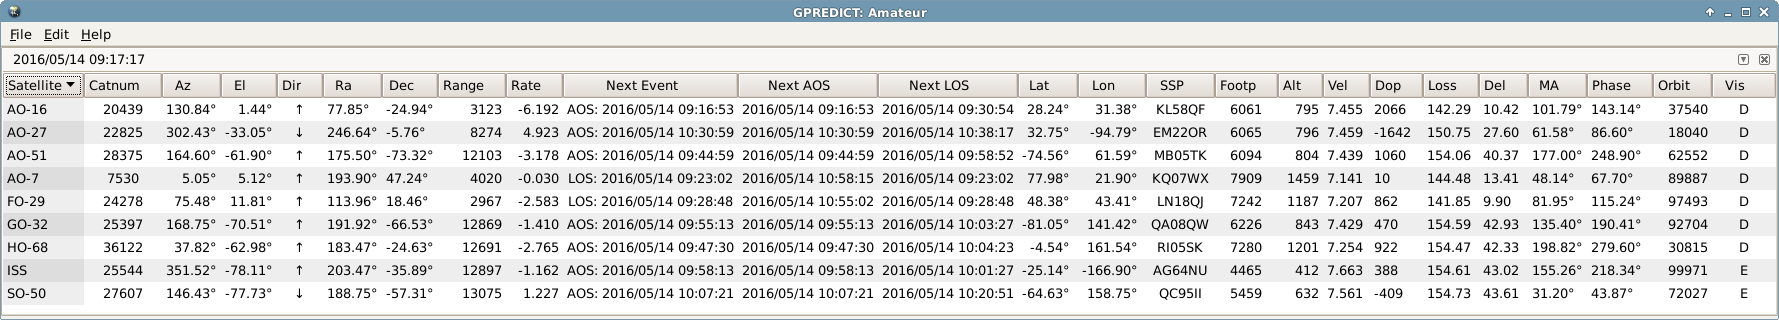
\includegraphics[width=1\textwidth]{listview}
	\caption{Listenansicht bzw. \myemph{List View} von GPredict}
	\label{fig:listview} 
\end{figure}

\textbf{Upcoming Passes View}\\
Die \myemph{Upcoming Passes View} (siehe Abbildung \ref{fig:upcomingpassesview}) zeigt alle Satelliten des aktuellen Moduls, deren Azimut und Elevation, sowie die Zeit bis zum nächsten Verschwinden des Satelliten, dem sogenannten \myemph{\ac{LOS}} bzw. dem nächsten Auftauchen, auch \myemph{\ac{AOS}} genannt.

\begin{figure}[h]
	\centering
	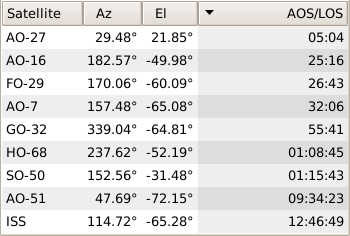
\includegraphics[width=0.3\textwidth]{upcomingpassesview}
	\caption{Upcoming Passes View}
	\label{fig:upcomingpassesview} 
\end{figure}

\clearpage

\subsection{Weitere Ansichten}

Bei allen Ansichten kann durch einen Klick auf den Satellitennamen (bei der \myemph{Single-Satellite View} ein Klick auf das Dreieck neben dem Namen) ein kleines Pop-Up Menü geöffnet werden, welches den entsprechenden Satellitennamen, die Option \myemph{Show next pass} und die Option \myemph{Future passes} anzeigt.

\begin{figure}[h]
	\centering
	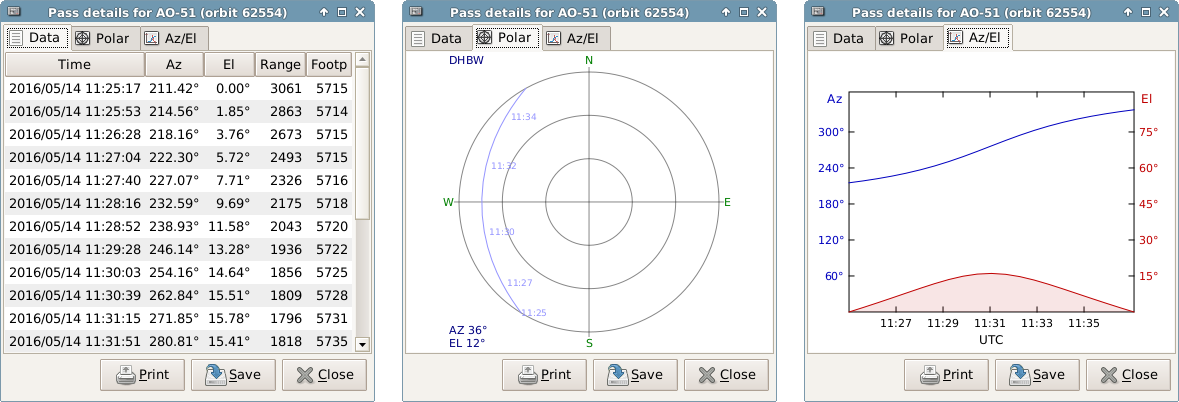
\includegraphics[width=1\textwidth]{passdetails}
	\caption{Pass Details}
	\label{fig:passdetails} 
\end{figure}

\begin{figure}[h]
	\centering
	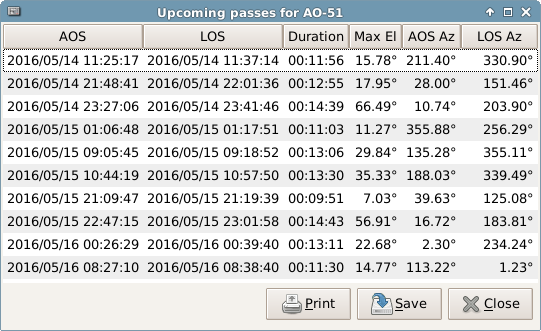
\includegraphics[width=0.5\textwidth]{upcomingpasses}
	\caption{Upcoming Passes}
	\label{fig:upcomingpasses} 
\end{figure}

\begin{figure}[h]
	\centering
	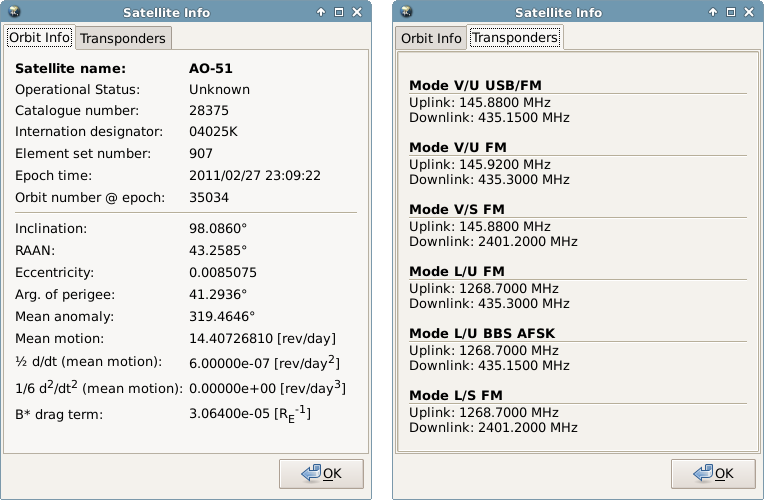
\includegraphics[width=0.7\textwidth]{satinfo}
	\caption{Satellite Info}
	\label{fig:satinfo} 
\end{figure}

\clearpage

\subsection{Modul Pop-Up Menü}

\begin{itemize}
	\parskip0pt
	\item \textbf{Antenna Control (Rotoren):} (noch kein Bild vorhanden)
	\item \textbf{Radio Control} (noch kein Bild vorhanden)
	\item \textbf{Sky at a Glance} (theskyataglance.png)
	\item \textbf{Time Controller} (timecontroller.png)
	\item \textbf{Modul-Einstellungen} (editmodule.png)
\end{itemize}

\subsection{GPredict Einstellungen}

\begin{itemize}
	\parskip0pt
	\item \textbf{General}
	\item \textbf{Modules}
	\item \textbf{Interfaces}
	\item \textbf{Predict}
\end{itemize}


\iffalse
\textbf{Map View}\\
alskfjlöajsf aöfljasldkfj laksjf lkad fasd\newpar
\textbf{Polar View}\\
öasjf lasj lkösda fj lfk kajj dj lk fas 
\fi

\clearpage

\section{HamLib-Programmierschnittstelle}

\begin{figure}[h]
	\centering
	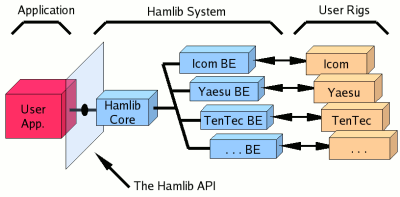
\includegraphics[width=0.5\textwidth]{hamlib}
	\caption{HamLib Design \cite{hamlib}}
	\label{fig:hamlib} 
\end{figure}

\section{Inbetriebnahme unter Windows}

Dieser Text soll ein Test sein, ob die .tex File auch online bearbeitet werden kann.

\section{Inbetriebnahme unter Linux}
